\section{Results}
\label{sec:results}

Unless stated otherwise, numbers are for SWE-bench Lite with gold files and their imports as candidates (\stat{lite:instances_with_gold_function} issues with a gold function), and intervals are 95\% bootstrap intervals over issues.

\subsection{Main comparison}

\begin{table*}[t]
\caption{SWE-bench Lite, gold files + direct imports. Gold-function recall at three budgets with 95\% intervals, and other metrics at the 25\% budget. All values in percent.}
\label{tab:main}
\centering
\footnotesize
\resizebox{\textwidth}{!}{\T{lite_oracle_imports_main}}
\end{table*}

\begin{figure*}[t]
\centering
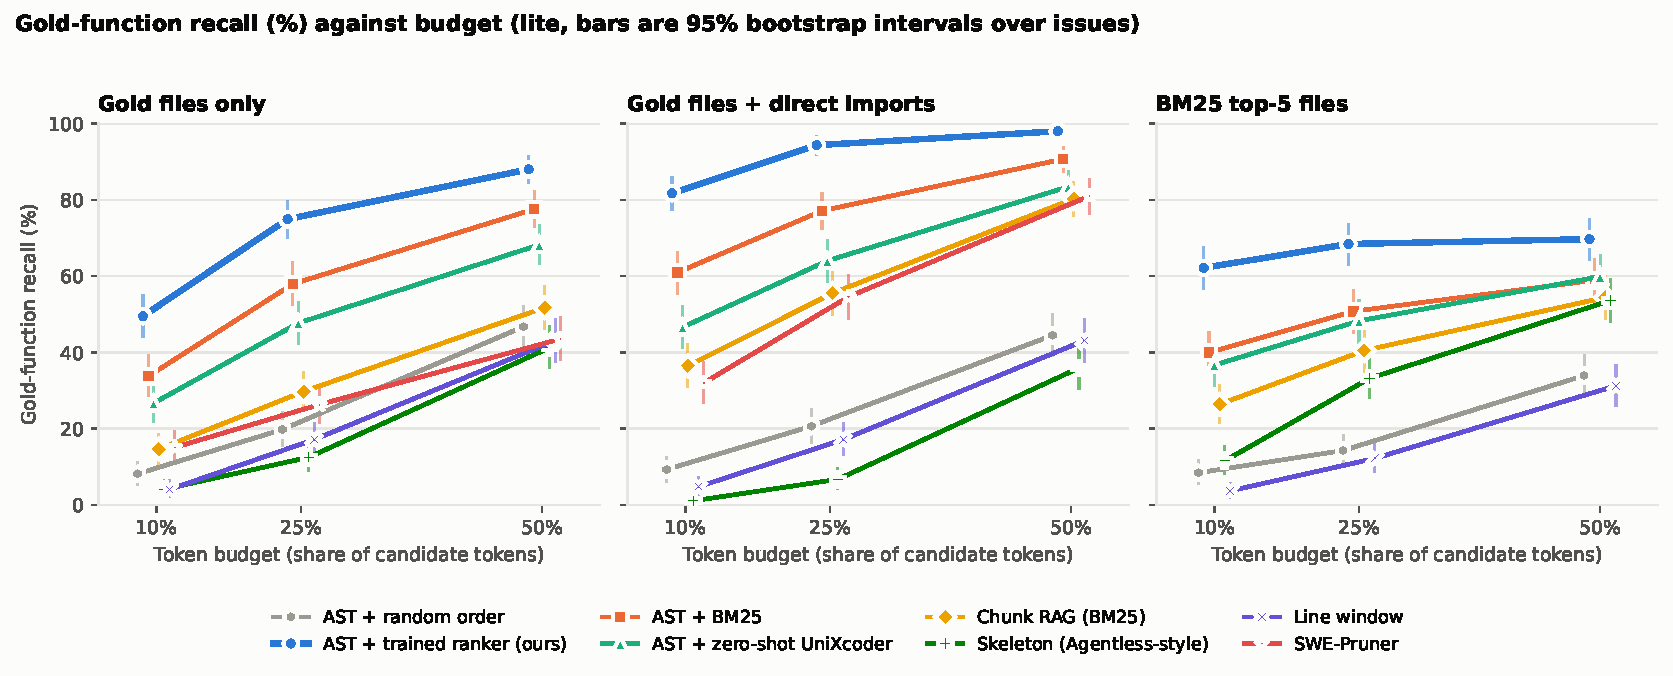
\includegraphics[width=\textwidth]{lite_recall_vs_budget}
\caption{Gold-function recall against budget on SWE-bench Lite under three ways of choosing candidate files. Bars are 95\% bootstrap intervals. In the BM25 panel, a gold function whose file was not retrieved counts as lost for every method.}
\label{fig:curves}
\end{figure*}

Table~\ref{tab:main} and Figure~\ref{fig:curves} give the main result.

\paragraph{RQ1: how much can be cut} With the trained ranker, cutting 90\% of the candidate tokens loses \emph{some} gold function in about one issue out of five (recall \res{lite:oracle_imports:ast_trained:r0.10:gold_fn_recall}\%), cutting 75\% keeps \res{lite:oracle_imports:ast_trained:r0.25:gold_fn_recall}\%, and cutting half keeps \res{lite:oracle_imports:ast_trained:r0.50:gold_fn_recall}\%. In absolute terms, a view of 4{,}000 tokens keeps \res{lite:oracle_imports:ast_trained:f4000:gold_fn_recall}\% of gold functions and one of 1{,}000 tokens keeps \res{lite:oracle_imports:ast_trained:f1000:gold_fn_recall}\%. How much can be cut therefore depends strongly on how units are ranked: a random order over the same units keeps \res{lite:oracle_imports:ast_random:r0.25:gold_fn_recall}\% at the 25\% budget, close to the budget itself, as it should be.

When only the gold files are candidates, every unit competes with units from the right file and the same relative budget is a much smaller number of tokens. Recall is lower for all methods (trained ranker \res{lite:oracle:ast_trained:r0.10:gold_fn_recall}\% at 10\% and \res{lite:oracle:ast_trained:r0.25:gold_fn_recall}\% at 25\%), and the order of methods is unchanged.

\paragraph{RQ2: does training help} Yes. The trained ranker and the zero-shot encoder differ only in their weights, and the paired difference in recall is \dif{lite:oracle_imports:ast_trained:ast_unixcoder:r0.10} points at the 10\% budget (interval \dif{lite:oracle_imports:ast_trained:ast_unixcoder:r0.10:lo} to \dif{lite:oracle_imports:ast_trained:ast_unixcoder:r0.10:hi}). Against BM25 on the same units, the stronger of the two cheap untrained scorers, the difference is \dif{lite:oracle_imports:ast_trained:ast_bm25:r0.10} points at 10\% (\dif{lite:oracle_imports:ast_trained:ast_bm25:r0.10:lo} to \dif{lite:oracle_imports:ast_trained:ast_bm25:r0.10:hi}), \dif{lite:oracle_imports:ast_trained:ast_bm25:r0.25} at 25\% (\dif{lite:oracle_imports:ast_trained:ast_bm25:r0.25:lo} to \dif{lite:oracle_imports:ast_trained:ast_bm25:r0.25:hi}) and \dif{lite:oracle_imports:ast_trained:ast_bm25:r0.50} at 50\% (\dif{lite:oracle_imports:ast_trained:ast_bm25:r0.50:lo} to \dif{lite:oracle_imports:ast_trained:ast_bm25:r0.50:hi}). The gap shrinks as the budget grows, as H2 predicted: with enough room, a mediocre ranking still reaches the right function.

It is worth noting that the untrained encoder is \emph{worse} than BM25. A general code encoder has no reason to map a bug report close to the function that causes the bug. Issues and functions often share identifiers, which BM25 exploits directly. Fine-tuning turns the encoder from the weakest reasonable scorer into the strongest, so the benefit comes from the task-specific supervision and not from using a neural model as such.

\paragraph{A larger model without training} AST + LLM perplexity ranks the same units by LongCodeZip's criterion, how much a unit lowers the perplexity of the issue under Qwen2.5-Coder-1.5B, a model about twelve times the size of ours. It is the strongest training-free scorer at the 10\% and 25\% budgets (\res{lite:oracle_imports:ast_ppl:r0.10:gold_fn_recall}\% and \res{lite:oracle_imports:ast_ppl:r0.25:gold_fn_recall}\%, against \res{lite:oracle_imports:ast_bm25:r0.10:gold_fn_recall}\% and \res{lite:oracle_imports:ast_bm25:r0.25:gold_fn_recall}\% for BM25), so a code model does carry some signal about where a bug sits. The paired difference to the trained ranker is still \dif{lite:oracle_imports:ast_trained:ast_ppl:r0.25} points at 25\% (\dif{lite:oracle_imports:ast_trained:ast_ppl:r0.25:lo} to \dif{lite:oracle_imports:ast_trained:ast_ppl:r0.25:hi}) and \dif{lite:oracle_imports:ast_trained:ast_ppl:r0.10} at 10\%, in favour of the trained ranker. It also scores a file in \res{lite:oracle_imports:ast_trained:r0.25:prep_ms_per_file}\,ms on average, where the perplexity ranking needs \res{lite:oracle_imports:ast_ppl:r0.25:prep_ms_per_file}\,ms.

\paragraph{RQ3: does granularity help} On the primary metric, clearly. BM25 over syntax-tree units keeps \dif{lite:oracle_imports:ast_bm25:chunk_bm25:r0.10} points more gold functions than BM25 over chunks at the 10\% budget (\dif{lite:oracle_imports:ast_bm25:chunk_bm25:r0.10:lo} to \dif{lite:oracle_imports:ast_bm25:chunk_bm25:r0.10:hi}) and \dif{lite:oracle_imports:ast_bm25:line_window:r0.10} more than a line window. The scorer is the same in the first comparison, so the difference is due to the unit.

This needs a qualification. Gold-function recall requires every line of a function to survive, and a chunk boundary inside a function makes that fail even when the edited line is kept. On gold-line recall, which has no such requirement, chunk BM25 and AST BM25 are level at the 25\% budget (\res{lite:oracle_imports:chunk_bm25:r0.25:gold_line_recall}\% and \res{lite:oracle_imports:ast_bm25:r0.25:gold_line_recall}\%). So syntax-tree units do not find the edited location more often than chunks do under the same scorer. What they add is that the function arrives whole and the view is valid code: \res{lite:oracle_imports:chunk_bm25:r0.25:parse_rate}\% of chunk views parse, against 100\% of ours. H1 holds as stated in the proposal, and this is the honest reading of why. The trained ranker is ahead on both metrics (\res{lite:oracle_imports:ast_trained:r0.25:gold_line_recall}\% line recall at 25\%).

\paragraph{The skeleton} The Agentless-style skeleton has near-perfect signature recall and very low full recall at tight budgets, because signatures of every unit consume most of the budget. It is a good first view for a model that will ask for more, and a poor final one.

\paragraph{Rank fusion} We expected that fusing BM25 ranks with the trained ranker's ranks would combine lexical and learned evidence. It does not help: the fusion is \res{lite:oracle_imports:ast_hybrid:r0.10:gold_fn_recall}\% at the 10\% budget against \res{lite:oracle_imports:ast_trained:r0.10:gold_fn_recall}\% for the trained ranker alone. The same pattern appeared on dev, where the decision to ship the trained ranker alone was made. A plausible reason is that the ranker was trained against BM25-selected negatives, so it has already learned to correct BM25's typical mistakes, and averaging the two brings those mistakes back.

\subsection{Second test set and retrieved files}

\begin{table}[t]
\caption{Gold-function recall (\%) at a 25\% budget for every candidate setting. Top: Lite. Bottom: Verified.}
\label{tab:settings}
\centering
\scriptsize
\setlength{\tabcolsep}{2.5pt}
\resizebox{\columnwidth}{!}{\T{lite_settings}}\\[4pt]
\resizebox{\columnwidth}{!}{\T{verified_settings}}
\end{table}

Table~\ref{tab:settings} repeats the comparison on SWE-bench Verified and with files retrieved by BM25. On Verified (\stat{verified:instances_with_gold_function} issues, \stat{verified:gold_per_issue} gold functions per issue against \stat{lite:gold_per_issue} in Lite) the trained ranker keeps \res{verified:oracle_imports:ast_trained:r0.10:gold_fn_recall}\% of gold functions at 10\% and \res{verified:oracle_imports:ast_trained:r0.25:gold_fn_recall}\% at 25\%, and BM25 keeps \res{verified:oracle_imports:ast_bm25:r0.10:gold_fn_recall}\% and \res{verified:oracle_imports:ast_bm25:r0.25:gold_fn_recall}\%. The paired difference at 10\% is \dif{verified:oracle_imports:ast_trained:ast_bm25:r0.10} points (\dif{verified:oracle_imports:ast_trained:ast_bm25:r0.10:lo} to \dif{verified:oracle_imports:ast_trained:ast_bm25:r0.10:hi}). The all-gold rate, which is the stricter number for multi-function patches, is \res{verified:oracle_imports:ast_trained:r0.25:all_gold}\% for the trained ranker at 25\% against \res{verified:oracle_imports:ast_bm25:r0.25:all_gold}\% for BM25.

With retrieved files, recall is capped by file retrieval: a gold function in a file that BM25 did not return is lost for every method. With the top 5 files the trained ranker keeps \res{lite:bm25_5:ast_trained:r0.25:gold_fn_recall}\% at the 25\% budget and BM25 on units keeps \res{lite:bm25_5:ast_bm25:r0.25:gold_fn_recall}\%. The order of methods is the same as with gold files, with one exception. The skeleton does well here (\res{lite:bm25_5:skeleton:r0.25:gold_fn_recall}\%), because it fills bodies in file order and the files arrive in BM25 rank order, so it inherits the retriever's ranking.

\subsection{Selector ablations}
\label{sec:ablation}

\begin{table}[t]
\caption{Selector variants on Lite (\%). ``Sig.'' is signature recall.}
\label{tab:ablation}
\centering
\scriptsize
\setlength{\tabcolsep}{2.5pt}
\resizebox{\columnwidth}{!}{\T{lite_oracle_imports_ablation}}
\end{table}

Table~\ref{tab:ablation} varies one selector choice at a time. The choices themselves were made on dev. These are the corresponding test numbers.

\emph{Pooling the budget} is the choice that matters most. Giving each file its own share drops the trained ranker from \res{lite:oracle_imports:ast_trained:r0.10:gold_fn_recall}\% to \res{lite:oracle_imports:ast_trained_perfile:r0.10:gold_fn_recall}\% at the 10\% budget, since most of the budget is then spent on files that contain nothing relevant.

\emph{The signature tier} costs almost nothing in the default setting, where signatures only use budget left over after the full bodies: full recall is \res{lite:oracle_imports:ast_trained:r0.10:gold_fn_recall}\% with it and \res{lite:oracle_imports:ast_trained_nosig:r0.10:gold_fn_recall}\% without, while signature recall at 10\% rises from \res{lite:oracle_imports:ast_trained_nosig:r0.10:sig_recall}\% to \res{lite:oracle_imports:ast_trained:r0.10:sig_recall}\%. Reserving 15\% of the budget for signatures is a real trade: full recall at 10\% falls to \res{lite:oracle_imports:ast_trained_sig15:r0.10:gold_fn_recall}\% and signature recall rises to \res{lite:oracle_imports:ast_trained_sig15:r0.10:sig_recall}\%. Which side of that trade is better depends on whether the agent can ask again, which our offline evaluation cannot settle.

\emph{Ranking by probability per token}, the usual greedy rule for a knapsack, is slightly worse than ranking by score (\res{lite:oracle_imports:ast_trained_density:r0.10:gold_fn_recall}\% at 10\%). It favours small units, and gold functions are larger than the average unit.

\subsection{Training variance and the patch filter}
\label{sec:seeds}

\begin{table}[t]
\caption{Training variance: gold-function recall (\%) of the trained ranker on dev, where the checkpoint is chosen, and on Lite, gold files + direct imports. The runs differ only in the seed, and in the last row in the filter that drops training patches touching more than five functions.}
\label{tab:seeds}
\centering
\scriptsize
\setlength{\tabcolsep}{2.5pt}
\resizebox{\columnwidth}{!}{\T{lite_seeds}}
\end{table}

We trained the ranker twice more with other seeds, and once without the filter on patch size (Table~\ref{tab:seeds}). The seed barely matters. On Lite the three runs keep \stat{seeds:lite:r0.10:min} to \stat{seeds:lite:r0.10:max}\% of gold functions at the 10\% budget and \stat{seeds:lite:r0.25:min} to \stat{seeds:lite:r0.25:max}\% at 25\%, a spread far smaller than the gaps between methods. Without the filter the ranker trains on \stat{train:unfiltered:examples} examples instead of \stat{train:main:examples}. It is level with the seeded runs on Lite (\res{lite:oracle_imports:ast_trained@unfiltered:r0.25:gold_fn_recall}\% at 25\%) and about a point lower on dev at the 10\% budget (\res{dev:oracle_imports:ast_trained@unfiltered:r0.10:gold_fn_recall}\% against \stat{seeds:dev:r0.10:min} to \stat{seeds:dev:r0.10:max}\%). So the filter, which we added to keep noisy multi-function patches out of training, makes no measurable difference.
